\chapter{Implementation} \label{implementation}


\section{Overview}

This chapter details the implementation of a robotic mapping and image processing pipeline designed for spatial mapping with a Turtlebot4 robot. Leveraging the capabilities of the Spectacular AI SDK and ROS2, I developed a custom ROS2 node that performs real-time mapping on the Turtlebot4. This node captures environmental data and processes it to generate keyframe-based mapping suitable for autonomous navigation and further spatial analysis.

In addition to the mapping node, I implemented a secondary ROS2 node running on a laptop, responsible for saving images captured at keyframe intervals. This image-saving process allows for high-resolution image acquisition, preserving critical visual information for later post-processing. A post-process script subsequently cleans the image set by discarding blurry or overexposed images. This refined set of images is then used as input to the COLMAP photogrammetry software, which reconstructs a 3D point cloud model from the images.

To enhance the 3D model, I applied Gaussian splatting to generate a smooth, visually coherent representation of the mapped environment. This pipeline supports high-quality spatial mapping with applications in various robotic and industrial domains, providing accurate visual models essential for analysis and further computational tasks.

\section{Mapping}

After our experiments with RTAB-Map and nvblox (see Chapter~\ref{experiments_3d_mapping}) it became clear that they are not suitable for our expectations. Due to RTAB-Map's lag and frequent lose of track and NVIDIA Isaac VSLAM's (and nvblox's) hardware requirements we did not want to use them in the implementation of the mapping. On the other hand, the Spectacular AI SDK proved itself to be precise in our experiments (see Section~\ref{experiments_spai}) and we did not have to invest in additional hardware, so we decided to proceed with it in the implementation. 

I created a ROS2 workspace for the robot which has a package that contains my \verb|spectacularai_node|. The node is the core component of our mapping implementation and is responsible for generating and publishing spatial data essential for real-time SLAM (Simultaneous Localization and Mapping). The node, located within the \verb|spectacularai_depthai_turtlebot| package, is built with the Spectacular AI SDK, which offers precise Visual-Inertial Odometry (VIO) and SLAM capabilities optimized for robotic applications.

The node initializes several ROS2 publishers that communicate mapping and image data. Key topics include \verb|/slam/odometry| for publishing the estimated pose, \verb|/tf| for broadcasting the transformation tree, \verb|/slam/left| for transmitting image data from the left camera, \verb|/slam/keyframe| for transmitting keyframes, \verb|/slam/pointcloud| for 3D point cloud data, and \verb|/slam/camera_info| to share camera intrinsic information.

Key methods in \verb|spectacularai_node| are as follows:
\begin{itemize}
    \item \verb|processOutput|: Monitors the VIO session output and processes each available frame.
    \item \verb|onVioOutput|: Called for each VIO output, publishing the odometry and TF data based on the calculated pose, which includes both position and orientation in the world frame.
    \item \verb|onMappingOutput|: This callback handles mapping outputs, iterating through updated keyframes and invoking methods to store and publish them.
    \item \verb|newKeyFrame|: Extracts pose and image data from keyframes, publishing each frame as a ROS2 message. The keyframe pose is converted to \textit{PoseStamped} format, while left-camera images are published via the \textit{CvBridge}.
    \item \verb|publishPointCloud|: Computes a 3D point cloud using position data transformed by the camera’s pose matrix. This point cloud is then published as a \textit{PointCloud2} message, enriched with color data if available.
\end{itemize}

After launching the node on the robot we got an error that the Spectacular AI Python SDK is not installed. We were not able to install it because, unless on \textit{x86} CPU architecture it is free, users have to pay for it to use on the \textit{aarch64} architecture (the robot's controller is a Raspberry Pi 4). After consulting with my advisor he suggested that I should ask the Spectacular AI Team if they would grant me the SDK for my thesis. I submitted a form on their website with my university e-mail address provided as my contact address and after a week they provided me the \textit{.whl} files of the Python SDK. I want to thank and give my best regards to the Spectacular AI Team and Jerry Ylilammi who gave me access to these files. With the Python SDK installed we were finally able to start the node successfully.

In addition to the robot’s workspace, a secondary ROS2 workspace was created specifically for a notebook situated on the Turtlebot4’s platform. This workspace comprises two main packages: \verb|rviz2_laptop| and \verb|keyframe_saver|. The \verb|rviz2_laptop| package contains a launch file to initiate RViz, allowing for real-time visualization of data generated by the \verb|spectacularai_node|. This capability facilitates interactive monitoring and helps verify the mapping accuracy while the robot is in operation. The RViz visualized mapping of my mapping node can be seen on Figure~\ref{fig:spai_mapping_rviz}

\begin{figure}[htbp]
	\centering
	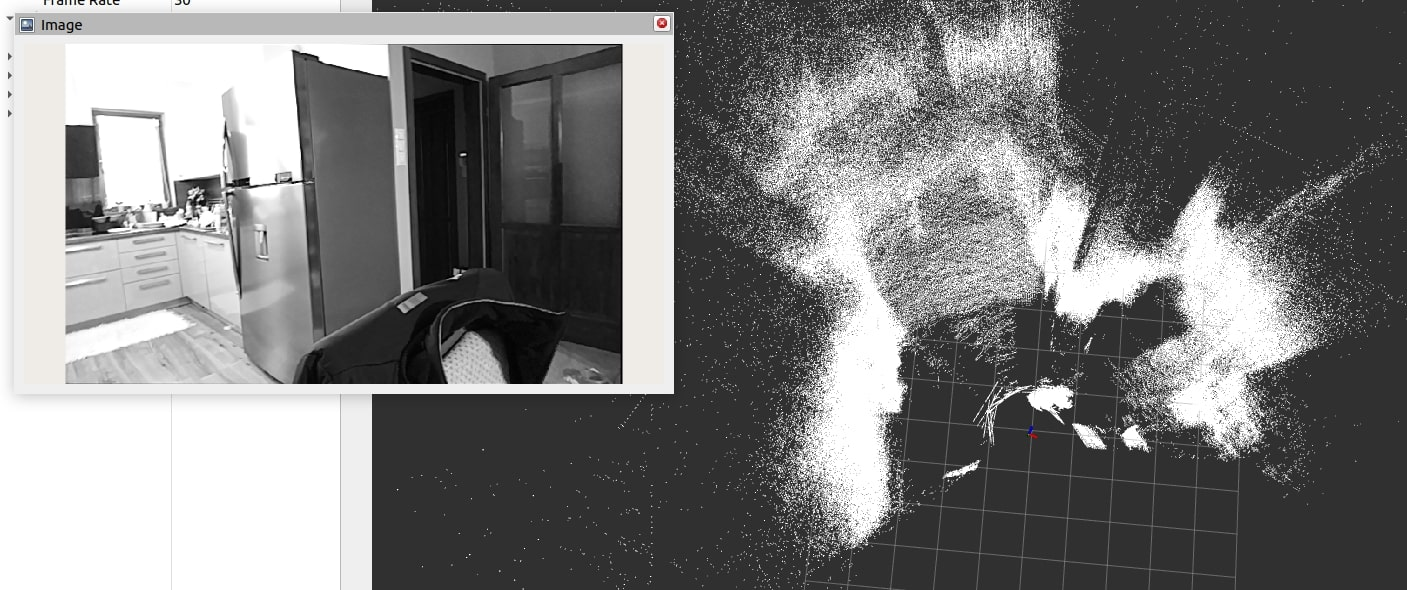
\includegraphics[width=150mm, keepaspectratio]{figures/spai_mapping_rviz.png}
	\caption{Mapping with Spectacular AI, visualized by RViz, point cloud from above}
	\label{fig:spai_mapping_rviz}
\end{figure}


\section{Saving and processing images for Gaussian splatting}

The second package, \verb|keyframe_saver|, implements a ROS2 node that subscribes to two topics: \verb|/slam/left| and \verb|/slam/keyframe|. This node, titled \textit{KeyframeImageSaver}, is responsible for capturing and saving images whenever a keyframe pose is detected, effectively archiving visual data throughout the robot’s mapping journey. The node’s code leverages OpenCV, alongside ROS2's \verb|cv_bridge|, to convert incoming ROS \textit{Image} messages to OpenCV-compatible images. When a new keyframe pose is received on the \verb|/slam/keyframe| topic, the node retrieves the latest image from \verb|/slam/left|, converts it, and stores it in a designated directory with a sequential filename.

This functionality is essential to the mapping workflow, as the saved images serve as the basis for further processing. The post-processing script used in this thesis further refines the keyframe images captured by the \textit{KeyframeImageSaver} node. By automatically identifying and discarding low-quality images — namely, those that are either blurry or overexposed — this script ensures that only high-quality images are retained for the photogrammetry reconstruction process. After filtering, the script renames the remaining images in a sequential order, which aids in organizing the dataset for subsequent processing steps.


\subsection{Blurry image detection}
To determine if an image is blurry, the script employs the variance of the Laplacian method~\cite{blur_detection}. This method calculates the variance of pixel intensity in the Laplacian of the grayscale version of the image. The Laplacian operator is defined as the sum of second-order partial derivatives:

\begin{equation}
 \triangle \mathit{f}\left (x,y  \right )= \frac{\partial^2 f }{\partial x^2} + \frac{\partial^2 f }{\partial y^2}
\end{equation}

where \(f(x,y)\) represents the grayscale image intensity at pixel location \((x,y)\). Variance measures the spread of values around the mean; a high variance indicates sharpness (high contrast edges), while a low variance suggests blurriness (low contrast edges). In this script, we define a threshold for variance: if the computed variance is below this threshold, the image is considered blurry and is flagged for deletion. 
The corresponding code snippet can be inspected here:

\FloatBarrier
\begin{lstlisting}[language=python,frame=single,float=!ht]
def is_blurry(image_path, threshold):
    """Check if an image is blurry using the variance of the Laplacian."""
    image = cv2.imread(image_path, cv2.IMREAD_GRAYSCALE)
    if image is None:
        return False
    laplacian_var = cv2.Laplacian(image, cv2.CV_64F).var()
    return laplacian_var < threshold
\end{lstlisting}
\FloatBarrier

In this function, \verb|cv2.Laplacian| calculates the Laplacian of the grayscale image, and \verb|.var()| computes the variance of the resulting matrix. If \verb|laplacian_var| is less than the threshold, the image is deemed blurry. I adjusted the threshold by doing experiments with blurry images, it performed best with the value of 500.

\subsection{Overexposed image detection}

For overexposure detection, the script evaluates the average brightness of an image. An overexposed image typically has a high overall intensity across the majority of pixels, indicating that many parts of the image are too bright. This approach converts the image to grayscale and calculates the mean pixel value. If the mean brightness exceeds a predefined threshold, the image is considered overexposed.

The mathematical foundation here is based on calculating the mean of pixel intensities (\(I\)) in a grayscale image, which is computed as:
\begin{equation}
    \textbf{Mean Brightness} = \frac{1}{N}\sum_{i=1}^{N} I\left ( i \right )
\end{equation}
where \(N\) is the total number of pixels in the image. A high mean value signifies overexposure.

The code for overexposure detection is as follows:

\FloatBarrier
\begin{lstlisting}[language=python,frame=single,float=!ht]
def is_overexposed(image_path, brightness_threshold):
    """Check if an image is overexposed based on brightness levels."""
    image = cv2.imread(image_path)
    if image is None:
        return False
    gray = cv2.cvtColor(image, cv2.COLOR_BGR2GRAY)
    mean_brightness = np.mean(gray)
    return mean_brightness > brightness_threshold
\end{lstlisting}
\FloatBarrier
Here, \verb|np.mean(gray)| computes the average brightness, and if this value exceeds the \verb|brightness_threshold|, the image is flagged for deletion. I adjusted the threshold by doing experiments with overexposed images, it performed best with the value of 200.

\subsection{Filtering and renaming}

After the detection of overexposed and blurry images the script iterates over all images in the specified directory, deletes any images identified as blurry or overexposed, and finally renames the remaining images in a sequential order. This ensures a clean, orderly dataset that is ready for the reconstruction pipeline.

By filtering out suboptimal images, this script plays a crucial role in optimizing the dataset, ensuring that the photogrammetry process has a higher chance of generating accurate 3D reconstructions. This refinement contributes to the overall quality and reliability of the map generated in the final stages of processing.

\subsection{COLMAP generation and Gaussian splatting}

With the filtered images we are almost ready for creating the Gaussian splat, the last thing that has to be done is generating a COLMAP from the images. It can be done using the \verb|ns-process-data| command from the nerfstudio (ns) suite to convert the processed images into a suitable format for Gaussian splatting. One example of its usage is as follows:

\FloatBarrier
\begin{lstlisting}[language=bash,frame=single,float=!ht]
ns-process-data images --data PATH/TO/keyframes --output-dir gsplat_input/
\end{lstlisting}
\FloatBarrier
where we need to specify that we want to use images as input, the path to them and the output path.

This step is crucial for adapting the images for use in NeRF-based training. The processing includes tasks like calculating camera intrinsics, generating point clouds, and constructing an appropriate input format for the Gaussian splatting training pipeline.

The next is step is to train the Gaussian splat model using the \verb|ns-train| command. The usage can be seen here:
\FloatBarrier
\begin{lstlisting}[language=bash,frame=single,float=!ht]
ns-train splatfacto-big --data gsplat_input/
\end{lstlisting}
\FloatBarrier

I prefer using the \verb|splatfacto-big| model because it creates more precise and realistic splats of the scenes compared to the default \verb|splatfacto| model. The command initiates the training of the Gaussian splat model on the processed data in the \verb|gsplat_input/| folder. After the training has started the process can be inspected via the viewer as seen on Figure~\ref{fig:training_nerf_karcag}.

This step is a core component of the pipeline, wherein the neural model learns to reconstruct scenes using Gaussian splatting. The model leverages the processed images to produce a probabilistic representation of the 3D environment, ideal for generating photorealistic splats.

When the training is complete, a created splat can be exported into a \verb|.ply| file with the following command:
\FloatBarrier
\begin{lstlisting}[language=bash,frame=single,float=!ht]
ns-export gaussian-splat --load-config outputs/gsplat_input/splatfacto/DATE/config.yml --output-dir exports/splat/\end{lstlisting}
\FloatBarrier
The saved file then can be opened with a Gaussian splat viewer and the created splat can be inspected.
